\documentclass[12pt, a4paper]{article}
\usepackage[print,sort]{standalone}
\usepackage[T1]{fontenc}
\usepackage[utf8]{inputenc}
\usepackage[english]{babel}
\usepackage{graphicx,float}
\usepackage{amssymb}
\usepackage{amsmath,cancel}
\usepackage{mathrsfs}
\usepackage{epstopdf}
\usepackage{subcaption}
\usepackage{slashed}
\usepackage{hhline}
\usepackage[margin=1.2in]{geometry}
\usepackage[hidelinks]{hyperref}
\usepackage{wrapfig}

\hfuzz=5pt

\begin{document}

\begin{titlepage}
\begin{center}
\vspace*{3cm}
\Huge
\textbf{Project 5} \\
\Large  
FYS4150 Computational Physics 
\vspace*{3cm} \\ 

Even S. Håland 
\vspace*{5cm} \\

\normalsize
\section*{Abstract}

In this project we study numerical and analytical solutions of the one- and two-dimensional diffusion 
equation. For the one-dimensional problem we implement three different methods; one explicit scheme 
(forward Euler) and two implicit schemes (backward Euler and Crank-Nicolson). We study the differences 
between them, as well as there stability, and how well they are able to approximate the analytical 
solution. We find (a bit surprisingly) that the backward Euler method is the one that is working best. 
For the two-dimensional problem we have only implemented an explicit solver, and we will see that this 
works fine as long as its stability condition is satisfied. 

\end{center}
\end{titlepage}

\section{Introduction}

The purpose of this project is to solve the partial differential equation (PDE) known as the 
diffusion equation (or heat flow equation), both in one and two dimensions\footnote{By  
dimensions we here mean spatial dimensions. The diffusion equation is also always time dependent.}. 
This equation has several applications in physics, and can for instance be used to describe the 
Brownian motion of particles and the heat flow in a material.   

The one-dimensional equation is given as 
\begin{align}
\frac{\partial ^2 u(x,t)}{\partial x^2} = \frac{\partial u(x,t)}{\partial t}, 
\label{eq:1d}
\end{align} 
where we have $t>0$ and $x\in [0,L]$, where we will choose $L=1$. In order to solve such a problem we 
also need an initial condition, which is given by 
\begin{align*}
u(x,0) = 0 \quad \text{for}  \quad 0<x<L, 
\end{align*} 
and boundary conditions, given as 
\begin{align*}
u(0,t) = 0 \:\: \text{and} \:\: u(L,t)=1 \quad \text{for} \quad t\geq 0.  
\end{align*}

The two-dimensional equation reads 
\begin{align}
\frac{\partial ^2 u(x,y,t)}{\partial x^2} + \frac{\partial ^2 u(x,y,t)}{\partial y^2} = 
\frac{\partial u(x,y,t)}{\partial t},  
\label{eq:2d}
\end{align}
where we also have $t>0$ and $x,y \in [0,L]$ with $L=1$. The initial condition is quite similar to the 
previous case:   
\begin{align*}
u(x,y,0) = 0 \quad \text{for}  \quad 0<x,y<L.  
\end{align*} 
However, the boundary conditions becomes slightly more complicated. It might be tempting to extend the 
boundaries from the one dimensional case such that $u(x,L,t)=u(L,y,t)=0$ and $u(L,y,t)=u(x,L,t)=1$. 
However, since the boundary is now a square in the $xy$-plane, this leaves us with some unpleasant 
discontinuities in two of the corners. This problem can be avoided by instead choosing boundary conditions 
\begin{align*}
u(0,y,t) & = u(x,0,t) = 0,  \\
u(L,y,t) & = y, \\ 
u(x,L,t) & = x, 
\end{align*}
where we always have $t\geq 0$, which gives a nice and continuous boundary. 

For the one dimensional case we will implement and study three different 
schemes for solving the equation numerically. These are the forward Euler, the backward Euler and the 
Crank-Nicolson schemes. In particular we will study the stability of these algorithms when varying the 
step size in space and time. For the two dimensional equation we will stick to one algorithm, which is 
an explicit scheme. In this case we will also study the stability of the algorithm. 

An important part of the project is also to solve equations \ref{eq:1d} and \ref{eq:2d} analytically, 
with the given initial and boundary conditions. The analytical solutions will be compared 
with the numerical ones in order to study the performance of our algorithms.   

We will start with the analytical solutions, before moving on to discussing the algorithms and how they 
are implemented. Finally we will look at (and discuss) the results. 

\section{Analytical solutions}

When solving the equations analytically we will, both in one and two dimensions, make use of the 
technique for solving PDE's known as separation of variables. That is we assume that the solution 
can be written as a product of functions, where each function only depends on one of the independent 
variables (i.e $x$, $y$ or $t$). In addition to this product we will add a term to our solution 
corresponding to the steady state solution. We will see that this last trick makes our lives quite a 
bit easier.  

Note also that both in this section and later we will use a short-hand notation for derivatives, 
reading 
\begin{align*}
f_x = \frac{\partial f}{\partial x} \quad \text{and} \quad f_{xx} = \frac{\partial^2 f}{\partial x^2}. 
\end{align*}

\subsection{One dimension}

For the one dimensional equation (eq. \ref{eq:1d}) we assume that the solution can be written as 
\begin{align*}
u(x,t) = F(x)T(t) + u_s(x), 
\end{align*}
where $u_s(x)$ is the steady state solution, which naturally is independent of time. We know that the 
steady state solution will be a straight line, i.e. $u_s(x)=x$, with the given boundaries. 

Inserting our proposed $u(x,t)$ into the diffusion equation leaves us with 
\begin{align*}
F_{xx} T = F T_t \quad \Rightarrow \quad \frac{F_{xx}}{F} = \frac{T_t}{T}, 
\end{align*} 
where each side of the latter equation must be a constant, which we (for later convenience) will call 
$-\lambda^2$. This means that we have two (ordinary) differential equations to solve: 
\begin{align*}
F_{xx} + \lambda^2 F = 0 \quad \text{and} \quad T_t = -\lambda^2 T 
\end{align*}  
The general solutions to these equations are 
\begin{align*}
F(x) = A \cos(\lambda x) + B \sin (\lambda x)  \quad \text{and} \quad  T(t) = C e^{-\lambda^2t}, 
\end{align*}
where $A,B,C$ are constants. The first boundary condition, $u(0,t)=0$, implies that $B=0$, which leaves 
us with the preliminary solution 
\begin{align*}
u(x,t) = A' \sin(\lambda x) e^{-\lambda^2 t} + x,   
\end{align*}
where $A' = AC$. The second boundary condition, $u(L=1, t)=1$, gives 
\begin{align*}
A'\sin (\lambda) = 0.  
\end{align*}
(Remember that the exponential is never zero.)
Now we have two options. We can choose $A'=0$, but this gives a trivial and non-interesting solution. A 
more interesting alternative is to choose $\lambda = n\pi$, where $n=1,2,3,\dots$. This means 
that the general solution must be written as a (Fourier) series, 
\begin{align*}
u(x,t) = \sum_{n=1}^\infty A_n \sin(n\pi x) e^{-n^2\pi^2t} + x. 
\end{align*}  
In order to determine the Fourier coefficients, $A_n$, we can use the initial condition, $u(x,0)=0$, 
which gets rid of the time part, and we find that 
\begin{align*}
\sum_{n=1}^\infty A_n \sin(n\pi x) = -x. 
\end{align*}  
In e.g. ref. \cite{Rottmann} on can find the Fourier expansion 
\begin{align*}
x = 2 \sum_{n=1}^\infty \frac{(-1)^{n-1}}{n} \sin nx,   
\end{align*} 
from which we easily can find the coefficients we need by letting $x\rightarrow \pi x$. Our general 
solution then becomes 
\begin{align*}
u(x,t) = x - \frac{2}{\pi} \sum_{n=1}^\infty \frac{(-1)^{n-1}}{n} \sin(n\pi x) e^{-n^2\pi^2t}. 
\end{align*}

\subsection{Two dimensions}

The method for solving the two-dimensional equation (eq. \ref{eq:2d}) goes much in the same pattern, but 
there are some complications because of the extra dimension. Let us start by assuming that 
\begin{align*}
u(x,y,t) = F(x,y)T(t) + u_s(x,y). 
\end{align*}
The first complication we meet is that it is a bit more tricky to realise what the steady state solution 
must be. The only possibility I have been able to come up with in order to satisfy the boundary 
conditions is $u_s(x,y) = xy$. (We will see later that this also matches the numerical solution quite 
good.)  

We insert our $u(x,y,t)$ into the diffusion equation, and gets 
\begin{align*}
\frac{F_{xx}}{F} + \frac{F_{yy}}{F} = \frac{T_t}{T} = -\lambda^2, 
\end{align*}
where $\lambda$ again is a constant, and we see that the time dependent part gets exactly the same 
form as in one dimension. However, the spatial part becomes
\begin{align*}
F_{xx} + F_{yy} + \lambda^2 F = 0, 
\end{align*}
which is still a PDE, and we need to separate it further. Let us assume that $F(x,y) = G(x)H(y)$, giving 
\begin{align*}
G_{xx} H + G H_{yy} + \lambda^2 GH = 0 \quad \Rightarrow \quad 
\frac{G_{xx}}{G} = -  \frac{H_{yy}}{H} - \lambda^2  = -\kappa^2,  
\end{align*}
where $\kappa$ is a constant, hence 
\begin{align*}
G_{xx} + \kappa^2 G = 0 \quad \text{and} \quad H_{yy} + \nu^2 H = 0, 
\end{align*}
where $\nu^2 = \lambda^2 - \kappa^2$. These equations have the same form as the spatial part of the 1D 
problem, and we can also eliminate the cosine part of the solutions using the boundary conditions 
$u(0,y,t) = u(x,0,t) = 0$. This gives a preliminary solution of the form 
\begin{align*}
u(x,y,t) = A \sin(\kappa x) B \sin (\nu y ) e^{-\lambda^2 t} + xy,  
\end{align*}  
where $A,B$ are constants. Using the other boundary conditions we get (neglecting the time part) 
\begin{align*}
A \sin(\kappa)B\sin(\nu y) + y = y \quad \text{and} \quad A \sin(\kappa x)B\sin(\nu ) + x = x, 
\end{align*}
giving $\kappa = n \pi$ and $\nu = m\pi$, where $m,n=1,2,3,\dots$, (hence $\lambda^2 = (n^2 + m^2)\pi^2$), 
and the full solution as a double Fourier series 
\begin{align*}
u(x,y,t) = \sum_{n=1}^\infty A_n \sin(n\pi x) \sum_{m=1}^\infty B_m \sin(m\pi y) e^{-(n^2 +m^2)\pi^2 t}+xy.  
\end{align*} 
As for the one-dimensional case we can use the initial condition to determine the Fourier coefficients, 
and the general solution becomes 
\begin{align*}
u(x,y,t) = xy - \frac{4}{\pi^2} \sum_{n=1}^\infty \sum_{m=1}^\infty 
							 	\frac{(-1)^{n+m-2}}{nm} \sin(n\pi x)  \sin(m\pi y) e^{-(n^2 +m^2)\pi^2 t}.
\end{align*} 

\section{Algorithms and code}  

Having solved the equations analytically we will now move to the numerical part of the project, and 
discuss the algorithms we have implemented. All code written for the project is found in 
the following git repository: \vspace{0.5cm} \\ 
\fbox{
\href{https://github.com/evensha/FYS4150/tree/master/Project5/Programs}
{https://github.com/evensha/FYS4150/tree/master/Project5/Programs} 
} \vspace{0.5cm} \\ 
This repository contains four important programs/scripts: 
\begin{itemize}
\item \texttt{Diffusion\_1d.cpp}
\item \texttt{Diffusion\_2d.cpp}
\item \texttt{Diffusion\_1d.py}
\item \texttt{Diffusion\_2d.py}
\end{itemize}
The first two are the C++ programs used to solve the one and two dimensional diffusion equation
numerically, while the last two are python scripts used to plot and analyse the output from the 
C++ programs, as well as calculate the analytical solution(s). 

\subsection{One dimension}

For solving the one dimensional equation we have implemented three different algorithms, which will
be briefly described in the following. We always use equal step lengths, with the spatial step, $\Delta x$, 
given by 
\begin{align*}
\Delta x = \frac{1}{n+1},  
\end{align*}  
where $n$ is the number of steps we consider. Also for the time step, $\Delta t$, we will only consider 
equal step sizes, but when choosing the actual value of $\Delta t$ we should take into account the 
stability limit of the algorithm in question. 

Position and time are discretized as 
\begin{align*}
t_j & = j\Delta t \quad j\geq 0,  \\
x_i & = i \Delta x \quad 0 \leq i \leq n+1,  
\end{align*} 
giving 
\begin{align*}
u(x,t) = u(x_i, t_j) = u_{i,j}. 
\end{align*}

\subsubsection{Forward Euler}

With the forward Euler scheme we approximate the derivatives as  
\begin{align*}
u_t \approx \frac{u(x,t+\Delta t) - u(x,t)}{\Delta t} = \frac{u_{i,j+1}- u_{i,j}}{\Delta t}, 
\end{align*}
and 
\begin{align*}
u_{xx} \approx \frac{u(x+\Delta x) - 2 u(x,t) + u(x-\Delta x,t)}{\Delta x^2} 
			=  \frac{u_{i+1,j} + u_{i,j} - u_{i-1,j}}{\Delta x^2}. 
\end{align*}
The approximation of the time derivative is the standard forward Euler formula with truncation error 
$O(\Delta t)$, while the double derivative in $x$ is the three point formula with truncation error 
$O(\Delta x^2)$. 

Now we have approximations for both sides of the 1D diffusion equation, and a simple manipulation of 
the equation ($u_{xx} = u_t$) leads us to the expression 
\begin{align}
u_{i,j+1} = \alpha u_{i-j,j} + (1-2\alpha)u_{i,j} + \alpha u_{i+1,j},
\label{eq:FE}
\end{align}
where 
\begin{align*}
\alpha = \frac{\Delta t}{\Delta x^2}. 
\end{align*}
This is a very simple equation to implement, since the solution for a given time step only depends on 
the solution for the previous time step. This means that, with given initial and boundary conditions, 
the solutions can be calculated directly without any "fancy" mathematics, hence this is referred to as 
an explicit scheme. This does however come with a price, as the algorithm is stable only if 
\begin{align*}
\Delta t \leq \frac{1}{2} \Delta x^2, 
\end{align*}
meaning that we need small (and hence many) time steps. (A more careful discussion of stability limits, 
both for this scheme and the other ones, can be found for instance in ref. \cite{Lecture Notes}.) 
The algorithm is implemented in the function 
\texttt{Forward\_Euler} in the one-dimensional program. 

\subsubsection{Backward Euler}

With the backward Euler scheme the time derivative is approximated by the backward Euler formula  
\begin{align*}
u_t \approx \frac{u(x,t) - u(x,t-\Delta t)}{\Delta t} = \frac{u_{i,j}- u_{i,j-1}}{\Delta t}, 
\end{align*}
while $u_{xx}$ is approximated as previously. This leads to the expression 
\begin{align}
u_{i,j-1} = -\alpha u_{i-1,j} + (1+2\alpha) u_{i,j} - \alpha u_{i+1,j},    
\label{eq:BE}
\end{align}  
with $\alpha$ defined as previously. 
We call this an implicit scheme, since we determine $u$ at time $t_{j-1}$ based on $u$ at time $t_j$. 
This means that we can't implement this equation directly (like we did for the forward Euler method), but 
we rather need to implement a method for solving the equation (or set of equations). This can be done 
by realizing that we can write this as a linear algebra problem. We do this by introducing a vector 
$V_j$ containing $u_{i,j}$ at a given time $t_j$, i.e. 
\begin{align*}
V_j = \left( \begin{array}{c}
u_{1,j} \\ u_{2,j} \\ \vdots \\ u_{n-1,j}
\end{array} \right). 
\end{align*}
We don't include the boundary points, as these are known. It is then fairly easy to realize that 
equation \ref{eq:BE} can be rewritten as 
\begin{align*}
V_{j-1} = \hat{A} V_j, 
\end{align*}
where $\hat{A}$ is a tridiagonal matrix given by 
\begin{align*}
\hat{A} = \left( \begin{array}{cccccc}
1+2\alpha & -\alpha & 0 & \cdots & \cdots & 0 \\ 
-\alpha & 1+2\alpha & -\alpha & 0 & \cdots & \cdots \\
\cdots & \cdots & \cdots & \cdots & \cdots & \cdots \\ 
\cdots & \cdots & 0 & -\alpha & 1+2\alpha & -\alpha \\
0 & \cdots &  \cdots & 0 & -\alpha & 1+2\alpha 
\end{array} \right),  
\end{align*}
thus we find the values of $u$ at time $t_j$ by finding the inverse of $\hat{A}$, i.e. 
\begin{align*}
V_j = \hat{A}^{-1} V_{j-1}. 
\end{align*}
This problem can be solved by the Thomas algorithm, which first performs a Gauss elimination and then a 
backward substitution, in order to find each element of $V_j$. This method is implemented in the 
\texttt{Backward\_Euler} function in the code.   

As we in this scheme use similar approximations to the derivatives as in the forward Euler scheme, the 
truncation errors are the same, i.e. $O(\Delta t)$ and $O(\Delta x^2)$. This algorithm is however stable 
for \textit{all} choices of $\Delta t$ and $\Delta x$. 

\subsubsection{Crank-Nicolson}

Finally we will, for the one-dimensional case, also consider the Crank-Nicolson scheme. The expressions 
used for approximations of the derivatives in this scheme are based on Taylor series expansion 
around $t' = t+\Delta/2$ (instead of $t+\Delta t$ as usual), hence this is referred to as a time centred 
scheme. The expression for the time derivative now becomes 
\begin{align*}
u_t \approx \frac{u(x,t) - u(x,t-\Delta t)}{\Delta t} = \frac{u_{i,j}- u_{i,j-1}}{\Delta t}, 
\end{align*}
which is the same expression as for the backward Euler scheme, but the difference being that the 
truncation error is now reduced to $O(\Delta t^2)$, because of the time centring. This also leads to 
a slightly more complicated expression for $u_{xx}$, given by 
\begin{align*}
u_{xx} \approx \frac{1}{2}\left( \frac{u_{i+1,j} - 2u_{i,j} + u_{i-1,j}}{\Delta x^ 2} 
				+ \frac{u_{i+1,j+1} - 2u_{i,j+1} + u_{i-1,j+1}}{\Delta x^ 2}  \right),  
\end{align*} 
which has truncation error $O(\Delta x^2)$. Putting these approximations together leads to the expression 
\begin{align*}
- \alpha u_{i-1,j} + (2 + 2\alpha)u_{i,j} - \alpha u_{i+1,j} 
= \alpha u_{i-1,j-1} + (2-2\alpha) u_{i,j-1} + \alpha u_{i+1,j-1}, 
\end{align*}
with $\alpha$ defined as previously. This can be written on matrix form as 
\begin{align*}
(2 \hat{I} + \alpha \hat{B} ) V_j = (2\hat{I} - \alpha \hat{B})V_{j-1}, 
\end{align*}
where $\hat{I}$ is the identity matrix, $V_j$ is like defined in the previous section, and $\hat{B}$ is 
tridiagonal matrix given as 
\begin{align*}
\hat{B} = \left( \begin{array}{cccccc}
2 & -1 & 0 & \cdots & \cdots & 0 \\
-1 & 2 & -1 & 0 & \cdots & \cdots \\
\cdots & \cdots & \cdots & \cdots & \cdots & \cdots \\ 
\cdots & \cdots & 0 & -1 & 2 & -1 \\
0 & \cdots & \cdots & 0 & -1 & 2 
\end{array} \right). 
\end{align*}
We can then calculate $V_j$ as 
\begin{align*}
V_j =  (2\hat{I} + \alpha \hat{B})^{-1} (2\hat{I} - \alpha \hat{B})V_{j-1}, 
\end{align*}
which can again be solved by the Thomas algorithm, with only a few modifications compared to the  
backward Euler scheme. This is implemented in the \texttt{Crank\_Nicolson} function in the code, and this 
scheme is also stable for all choices of $\Delta x$ and $\Delta t$. 

\subsection{Two dimensions}

For the two dimensional diffusion equation we will only consider an explicit scheme, very similar to 
the forward Euler scheme described above, only with an extra space dimension. We now discretize 
$x,y,t$ by 
\begin{align*}
x_i = x_0 + ih, \quad y_j = y_0 + jh \quad\text{and} \quad t_l = t_0 + l\Delta t,  
\end{align*}
where $0\leq i,j\leq n+1$ and $l\geq 0$, with 
\begin{align*}
h = \frac{1}{1+n}, 
\end{align*}
meaning that we use the same step size in $x$- and $y$-direction. Using the same approximations for the 
derivatives as for the 1D forward Euler scheme we arrive to the explicit expression 
\begin{align*}
u_{i,j}^{l+1} = u_{i,j}^l + \alpha \left[ u_{i+1,j}^l + u_{i-1,j}^l + u_{i,j+1}^l + u_{i,j-1}^l
				-4 u_{i,j}^l  \right]. 
\end{align*}
This is implemented in \texttt{Forward\_Euler} function in the 2D program. (Notice that in this program 
I have also tried to implement the iterative Jacobi method for solving the implicit 2D scheme, without 
great success. I have however not spent a lot of time on figuring out what I have done wrong here, but 
rather decided to just stick to the explicit solver.)  

\section{Results}

All results are presented in the following section, including comparisons of the different schemes and 
comparisons with the analytical solution. 

\subsection{One dimension}

In one dimension we will study the solution two different time points, $t_1=0.05$ and $t_2=0.5$, where we 
have chosen these points so that the system is in "motion" at $t_1$, while at $t_2$ it has reached 
the steady state. We will also look at two different choices of $\Delta x$, and choose $\Delta t$ as 
dictated by the stability limit of the forward Euler method. 

The numerical solutions using each of the solvers are plotted together with the analytical solution 
in Figure \ref{fig:1d} for $t_1$ and $t_2$, using $\Delta x = 0.1$ in the upper plots and 
$\Delta x = 0.01$ in the lower plots. The 
information we are able to extract from these plots is however quite limited, as all solvers seem to 
give good agreement with the analytical solution. 

It might be more interesting to study Figure 
\ref{fig:1d_diff}, which shows the absolute value of the difference between the analytical solution and 
each of the numerical ones. Here we see that the solver that (in general) seems to be performing best is 
backward Euler. This is a bit surprising, as the truncation error in the Crank-Nicolson method should be
smaller, suggesting that there might be something slightly wrong with the implementation of the 
Crank-Nicolson algorithm. We also notice that the forward Euler solver shows some weird behaviour, but 
we have to keep in mind that the solution is obtained at the stability limit of this solver 
(i.e. $\Delta t = 1/2 \Delta x^2$). In Figure \ref{fig:1d_unstable} we can see the catastrophic 
consequences of increasing the time step by a factor of two, to $\Delta t = \Delta x^2$.        

\begin{figure}[ht!]
	\centering 
  	\begin{subfigure}[b]{0.495\textwidth}
		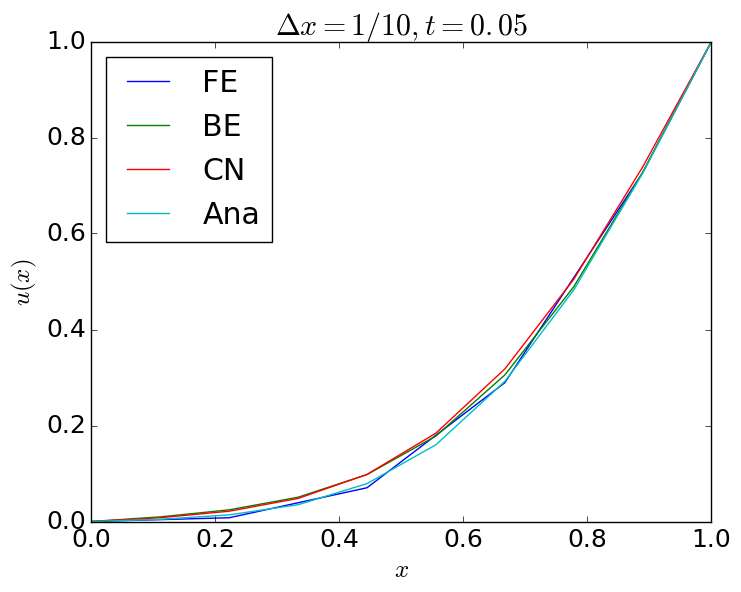
\includegraphics[width=\textwidth]{../Programs/Output/Diffusion_1d_9_t1.png}
        %\caption{}
        %\label{}
  	\end{subfigure}
  	\begin{subfigure}[b]{0.495\textwidth}
		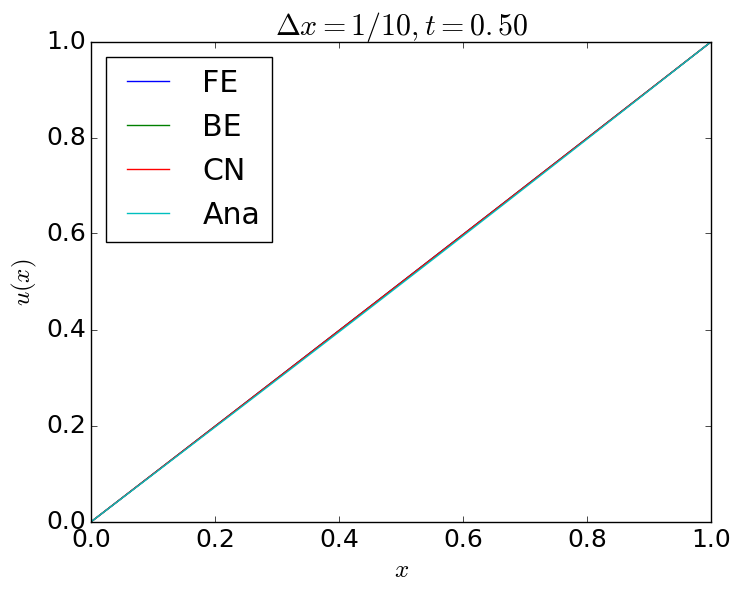
\includegraphics[width=\textwidth]{../Programs/Output/Diffusion_1d_9_t2.png}
        %\caption{}
        %\label{}
  	\end{subfigure}
  	\begin{subfigure}[b]{0.495\textwidth}
		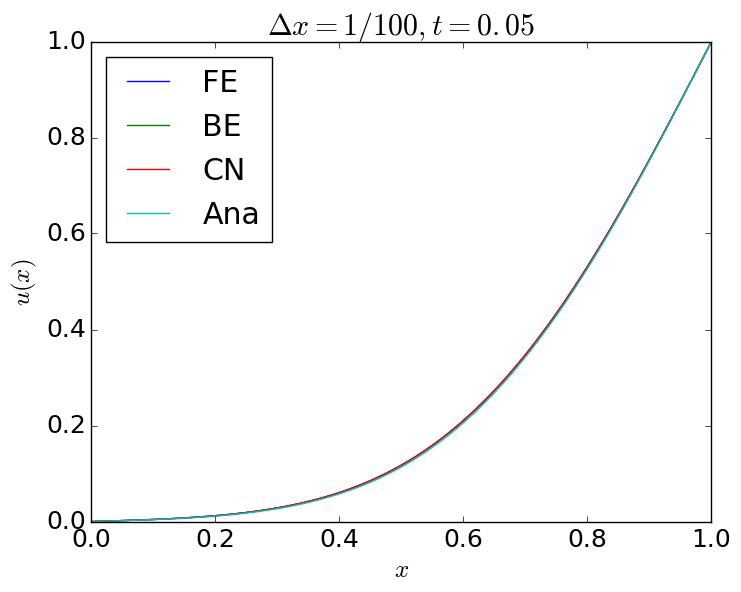
\includegraphics[width=\textwidth]{../Programs/Output/Diffusion_1d_99_t1.png}
        %\caption{}
        %\label{}
  	\end{subfigure}
  	\begin{subfigure}[b]{0.495\textwidth}
		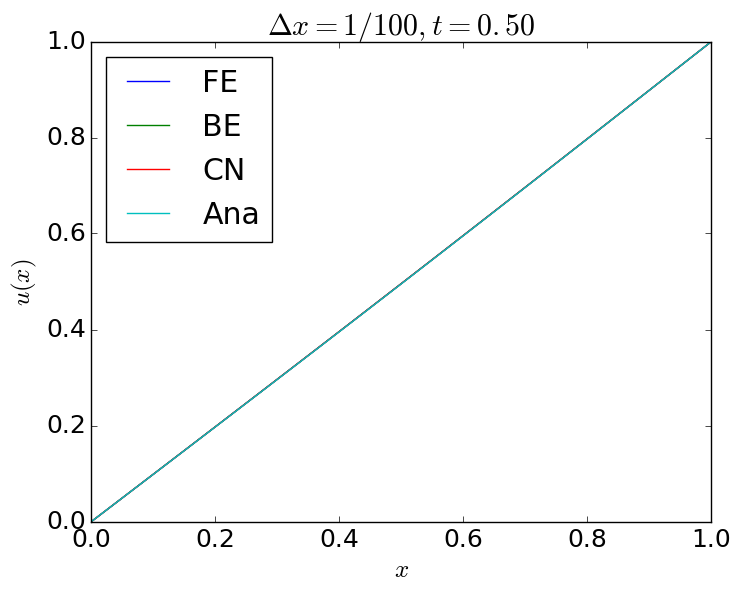
\includegraphics[width=\textwidth]{../Programs/Output/Diffusion_1d_99_t2.png}
        %\caption{}
        %\label{}
  	\end{subfigure}
  	\caption{Numerical and analytical solution for the 1D diffusion equation, using $\Delta x = 0.1$ 
  	in the upper plots and $\Delta x = 0.01$ in the lower plots.}
  	\label{fig:1d}	
\end{figure}


\begin{figure}[ht!]
	\centering 
  	\begin{subfigure}[b]{0.495\textwidth}
		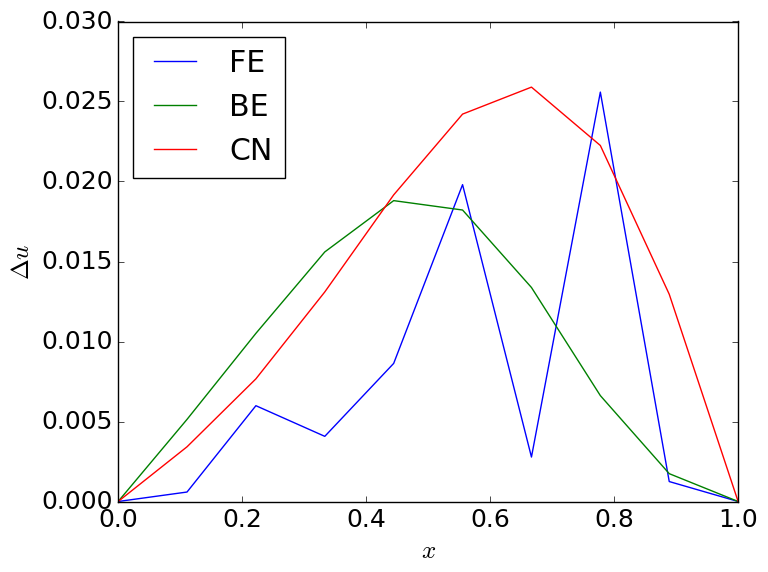
\includegraphics[width=\textwidth]{../Programs/Output/Delta_t1_1d_9.png}
        %\caption{}
        %\label{}
  	\end{subfigure}
  	\begin{subfigure}[b]{0.495\textwidth}
		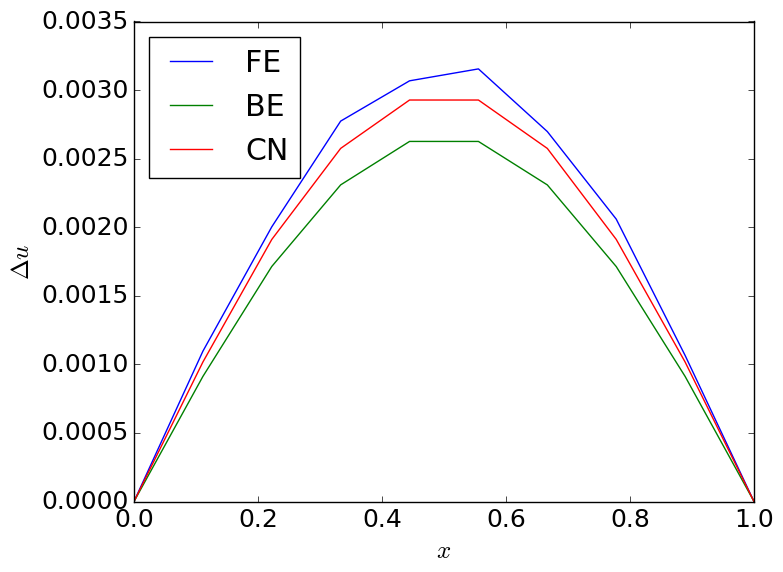
\includegraphics[width=\textwidth]{../Programs/Output/Delta_t2_1d_9.png}
        %\caption{}
        %\label{}
  	\end{subfigure}
  	\begin{subfigure}[b]{0.495\textwidth}
		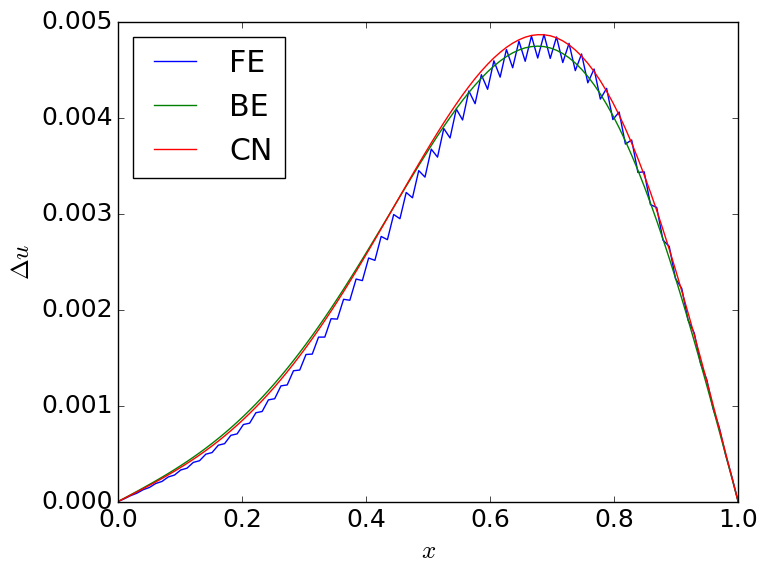
\includegraphics[width=\textwidth]{../Programs/Output/Delta_t1_1d_99.png}
        %\caption{}
        %\label{}
  	\end{subfigure}
  	\begin{subfigure}[b]{0.495\textwidth}
		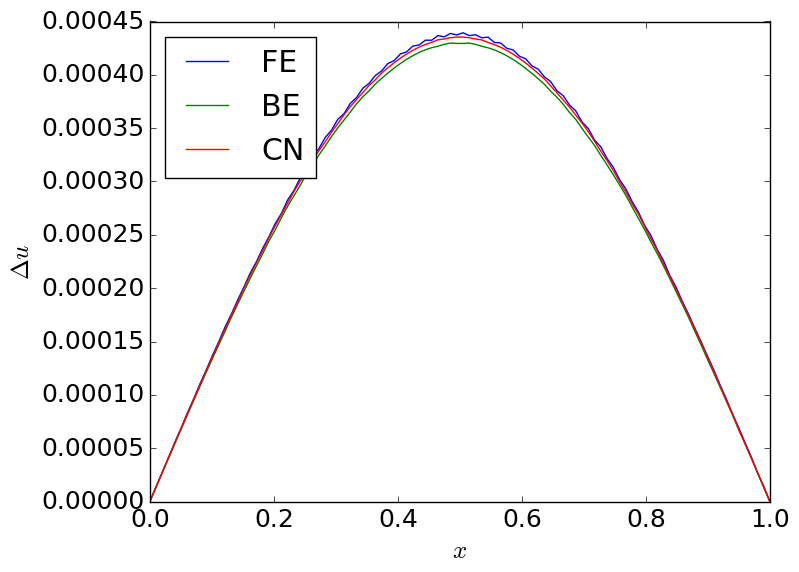
\includegraphics[width=\textwidth]{../Programs/Output/Delta_t2_1d_99.png}
        %\caption{}
        %\label{}
  	\end{subfigure}
  	\caption{Absolute differences ($\Delta u$) between numerical and analytical solution, 
  	using $\Delta x = 0.1$ in the upper plots and $\Delta x = 0.01$ in the lower plots.}
  	\label{fig:1d_diff}	
\end{figure}

\begin{figure}[ht!]
	\centering 
 	\begin{subfigure}[b]{0.495\textwidth}
		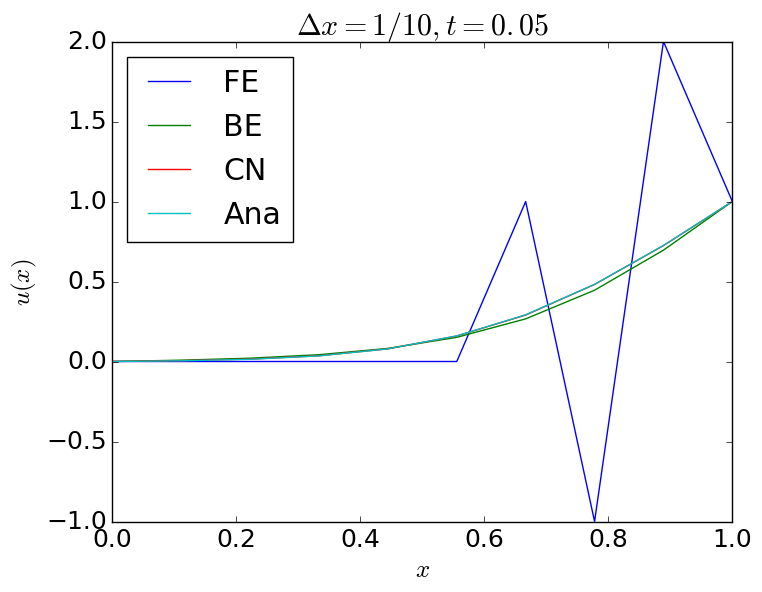
\includegraphics[width=\textwidth]{../Programs/Output/Diffusion_1d_t1_u.png}
        %\caption{}
        %\label{}
  	\end{subfigure}
  	\begin{subfigure}[b]{0.495\textwidth}
		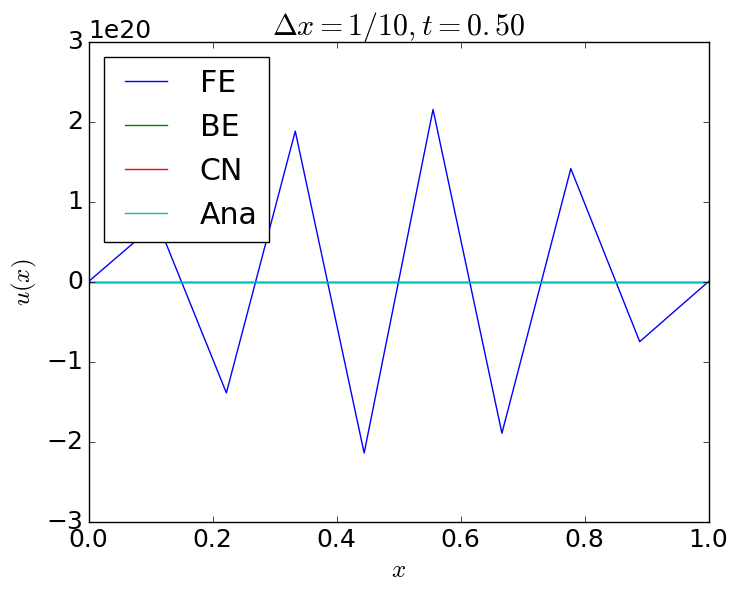
\includegraphics[width=\textwidth]{../Programs/Output/Diffusion_1d_t2_u.png}
        %\caption{}
        %\label{}
  	\end{subfigure}	
  	\caption{Diffusion equation solved using $\Delta t = \Delta x^2$, meaning that the forward Euler 
  	solver is (obviously) unstable.}
  	\label{fig:1d_unstable}
\end{figure}

\subsection{Two dimensions}

Also in two dimensions we consider two different time points, $t_1 = 0.01$ and $t_2 = 1.0$. We first 
consider $h=1/100$ and $\Delta t = h^2/2$ (i.e. the stability limit for the FE method). Solutions 
at these two times are shown in Figure \ref{eq:2d}. At $t_2$ we can see that the system has reached the 
steady state, since the surface has been "stretched out". In Figure \ref{fig:2d_delta} we see the 
absolute differences between the analytical solution and the numerical one. We see that (as for the 
one-dimensional problem) the approximation is better in the steady state, which seems natural as the 
slope is steeper and the "structure" of the surface is more complicated at $t_1$. It is also noteworthy 
that these plots suggests that our guess at the steady state solution was probably correct.       

\begin{figure}[ht!]
	\centering 
	\begin{subfigure}[b]{0.495\textwidth}
		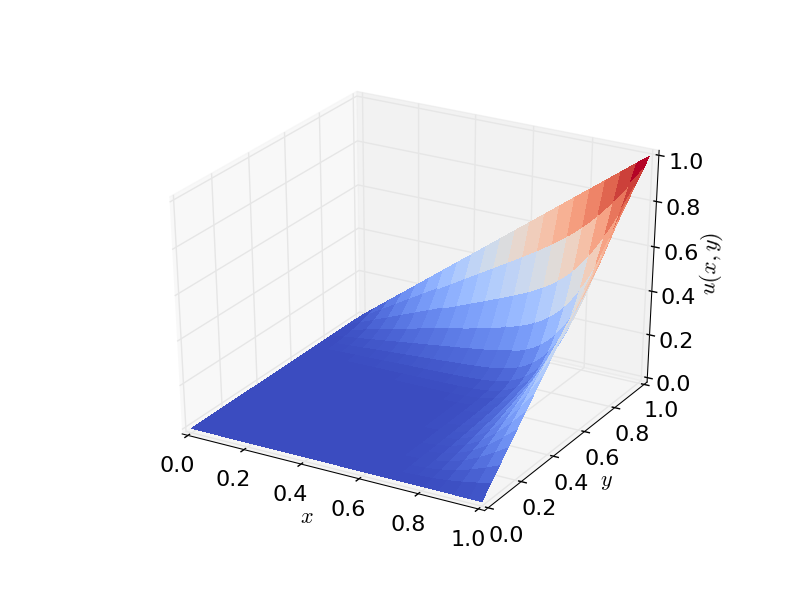
\includegraphics[width=\textwidth]{../Programs/Output/Diffusion_2d_t1.png}
        \caption{}
        %\label{}
  	\end{subfigure}
  	\begin{subfigure}[b]{0.495\textwidth}
		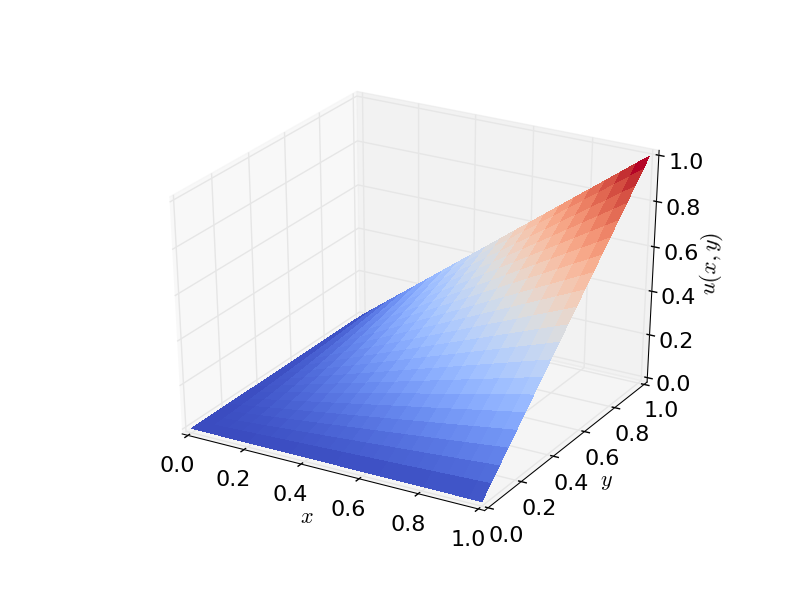
\includegraphics[width=\textwidth]{../Programs/Output/Diffusion_2d_t2.png}
        \caption{}
        %\label{}
  	\end{subfigure}	
  	\caption{Numerical solution to the 2D diffusion equation at two different times; 
  	(a) $t_1$ and (b) $t_2$.}
  	\label{fig:2d}
\end{figure}

\begin{figure}[ht!]
	\centering 
 	\begin{subfigure}[b]{0.495\textwidth}
		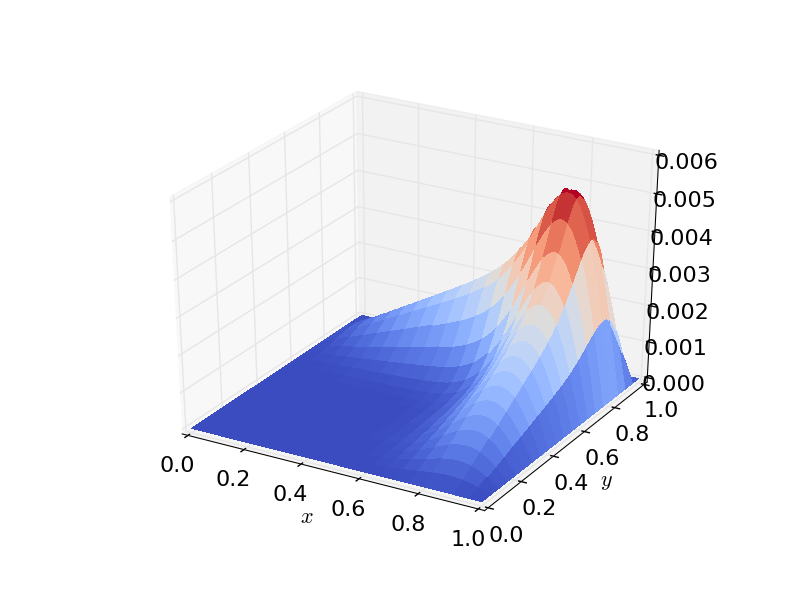
\includegraphics[width=\textwidth]{../Programs/Output/Delta_2d_t1.png}
        \caption{}
        %\label{}
  	\end{subfigure}
  	\begin{subfigure}[b]{0.495\textwidth}
		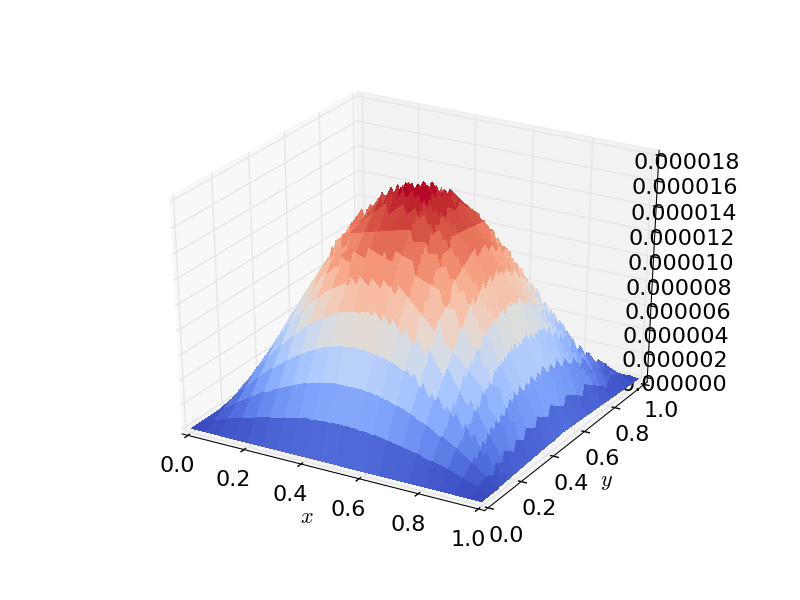
\includegraphics[width=\textwidth]{../Programs/Output/Delta_2d_t2.png}
        \caption{}
        %\label{}
  	\end{subfigure}	
  	\caption{Difference between analytical and numerical solutions for the 2D diffusion equation at 
  	two different times; (a) $t_1$ and (b) $t_2$.}
  	\label{fig:2d_delta}
\end{figure}

So we have now seen that we are able to approximate the analytical solution quite well with the 
explicit solver. The disadvantage of using the explicit solver is however, like we also saw in the 
one-dimensional case, that the stability requirement is quite strict. In Figure \ref{fig:2d_us} we 
see how the solution at $t_2$ look like when only slightly reducing the time step to 
$\Delta t = (1/1.99) h^2$. (Notice carefully the scale one the $z$-axis in this figure.) 

\begin{figure}
\begin{center}
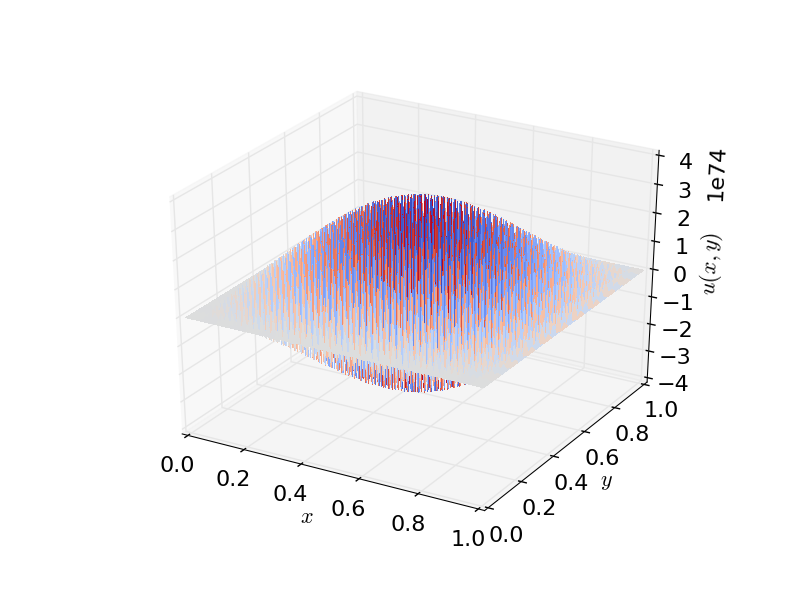
\includegraphics[scale=0.5]{../Programs/Output/Diffusion_2d_t2_us.png}
\caption{Numerical solution of the 2D diffusion equation at $t_2$ made with the explicit solver using 
$\Delta t = 1/1.99 h^2$.}
\label{fig:2d_us}
\end{center}
\end{figure}

\section{Summary and conclusions}

In this project we have solved the diffusion equation, both numerically and analytically, in one and 
two dimensions. For the one-dimensional problem we study three different solution schemes; the 
explicit forward Euler method, and the implicit backward Euler and Crank-Nicolson methods. We saw that 
the backward Euler was the one that seemed to be working best. We also saw that the advantage of the 
implicit solvers is that they are stable for any choices of step size, while the forward Euler solver 
has a strict stability requirement. 

For the two-dimensional problem we only implemented an explicit algorithm, and we saw that it gives 
good approximations to the numerical solution, as long as we stay within the stability limit.  

\begin{thebibliography}{40}

\bibitem{Rottmann} K. Rottman (2003). \textit{Matematisk formelsamling}, Spektrum forlag, Norway. 

\bibitem{Lecture Notes} M. Hjort-Jensen (2015), \textit{Computational Physics - Lecture Notes Fall 2015}, 
Department of Physics, University of Oslo. \\ 
\href{https://github.com/CompPhysics/ComputationalPhysics/blob/master/doc/Lectures/lectures2015.pdf}
{https://github.com/CompPhysics/ComputationalPhysics/blob/master\\/doc/Lectures/lectures2015.pdf}

\end{thebibliography}

\end{document}